% !TEX root = ../SU2-Scitech15.tex

\section{Results}
The flow past a NACA 0012 has been modeled using each one of the 5 meshes described at $0^\circ$, $10^\circ$ and $15^\circ$ angles of attack. To better understand the effect that the grid has in the flow solution and integrated forces, the pressure coefficients (Cp) for all the angles of attack simulated modeled using a limiter value of 0.1 have been plotted in Figure~\ref{fig:cp_lim0.1}.

\begin{figure}[]
  \begin{subfigmatrix}{2}
    \subfigure[$0^\circ$ Angle of Attack.]{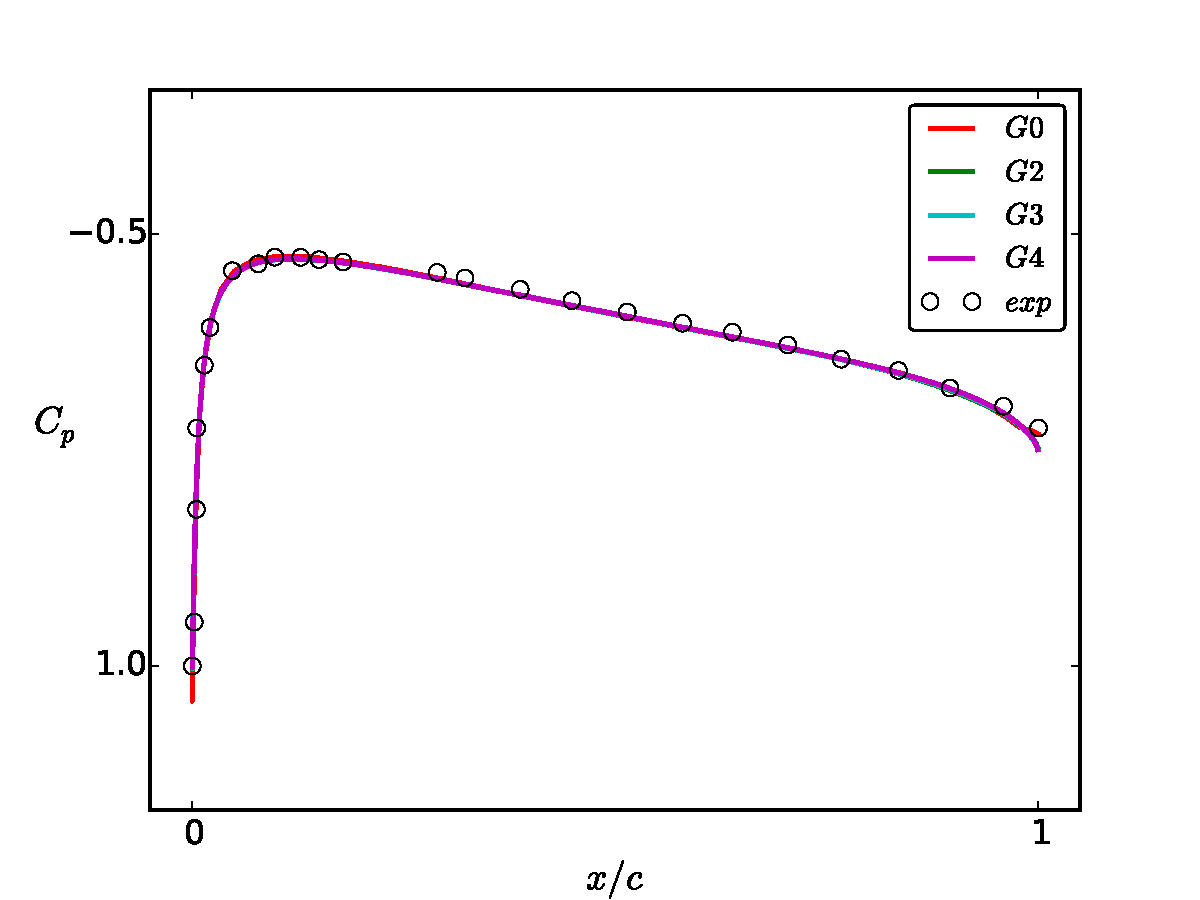
\includegraphics{Cp_vs_Grid_Lim_0_1_deg0.pdf}}
    \label{fig:cp_lim0.1_AoA0}
    \subfigure[$10^\circ$ Angle of Attack.]{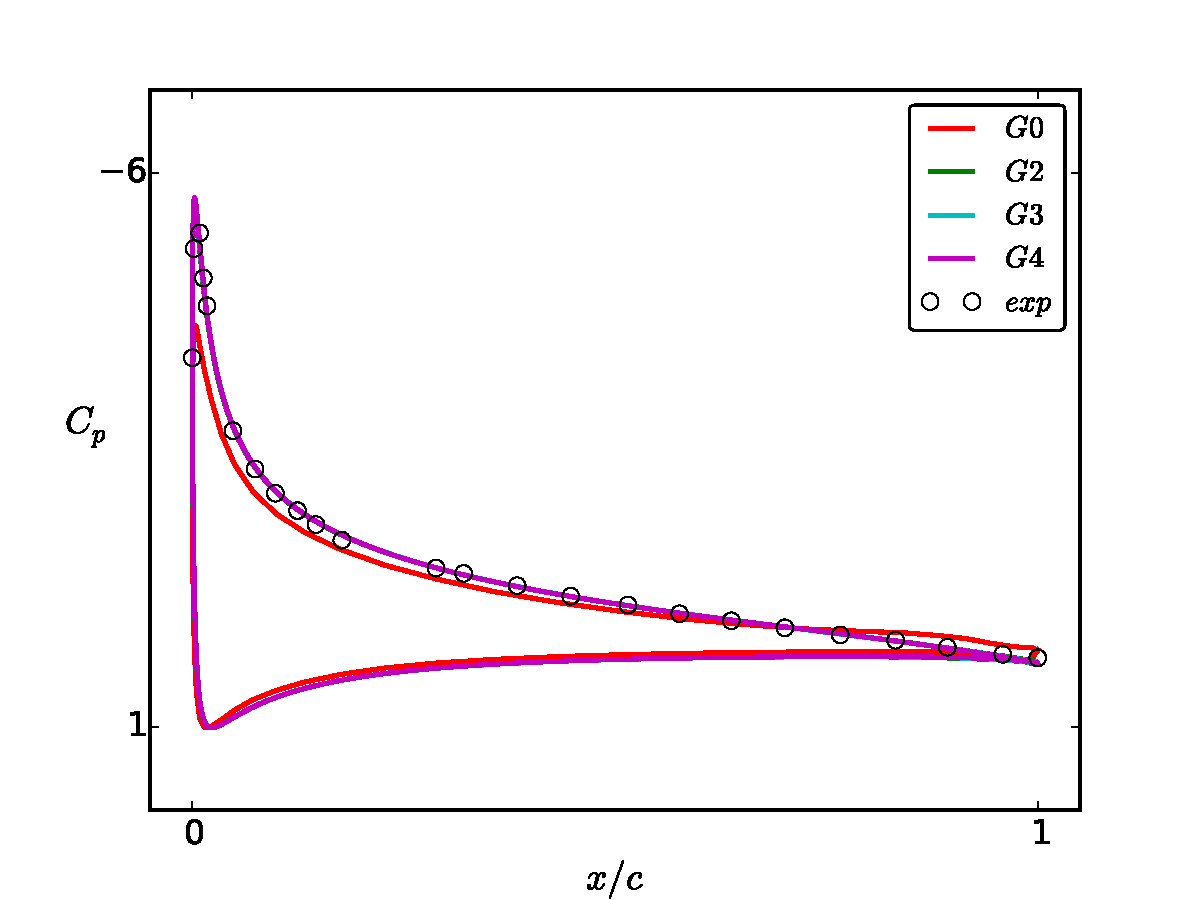
\includegraphics{Cp_vs_Grid_Lim_0_1_deg10.pdf}}
    \label{fig:cp_lim0.1_AoA10}
  \end{subfigmatrix}
  \begin{subfigmatrix}{1}
  	\subfigure[$15^\circ$ Angle of Attack.]{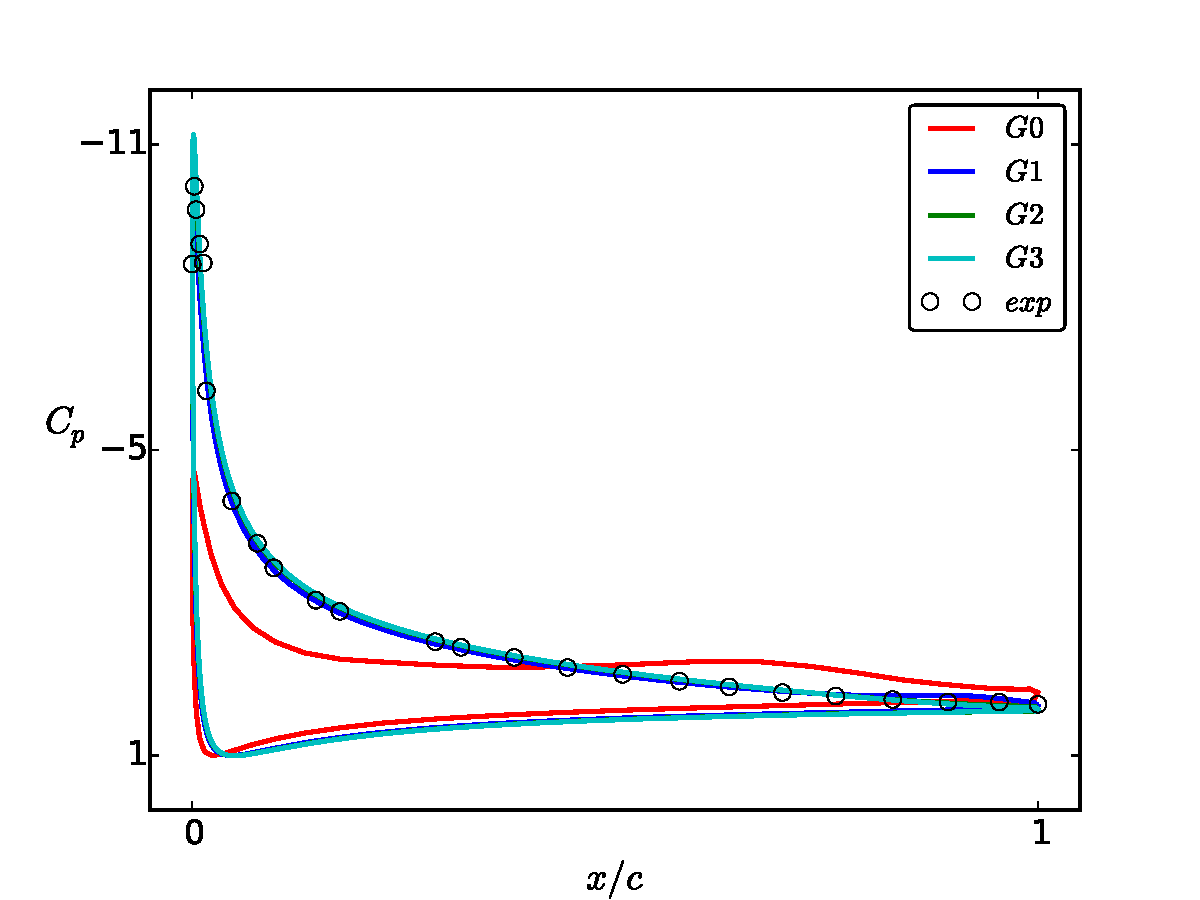
\includegraphics[width=.5\textwidth]{Cp_vs_Grid_Lim_0_1_deg15.pdf}}
    \label{fig:cp_lim0.1_AoA15}
  \end{subfigmatrix}
  
  \caption{Pressure coefficient of the NACA 0012 with a limiter value of 0.1 for 5 different grids.}
  \label{fig:cp_lim0.1}
\end{figure}

As can be expected, the Cp reflects that as the grid resolution increases Cp converges towards the experimental results. This behavior can be attributed to the lack of resolution mainly in the leading and trailing edges of the airfoil causing the miss prediction of the gradients and the flow structure.

Although it can be seen the that to achieve the correct solution, meshes such as G3 and G4 are adequate, there is a significant computational cost that has to be considered due to the high resolution involved. Keeping in mind the objective of this article to explore different alternatives to make the use of coarser grids for design purposes, various limiter values have been explored. 

\begin{figure}[]
%%% Not all this data was in the Google doc to be able to do the plot. %%%
%  \begin{subfigmatrix}{2}
%    \subfigure[$C_d$ Vs. limiter at $0^\circ$ Angle of Attack.]{\includegraphics{limiter_vs_drag_0deg.pdf}}
%    \label{fig:lim_drag_AoA0}
%    \subfigure[$C_l$ Vs. limiter at $0^\circ$ Angle of Attack.]{\includegraphics{limiter_vs_lift_0deg.pdf}}
%    \label{fig:lim_lift_AoA0}
%  \end{subfigmatrix}
%  \begin{subfigmatrix}{2}
%      \subfigure[$C_d$ Vs. limiter at $10^\circ$ Angle of Attack.]{\includegraphics{limiter_vs_drag_10deg.pdf}}
%      \label{fig:lim_drag_AoA10}
%      \subfigure[$C_l$ Vs. limiter at $10^\circ$ Angle of Attack.]{\includegraphics{limiter_vs_lift_10deg.pdf}}
%      \label{fig:lim_lift_AoA10}
%    \end{subfigmatrix}
    \begin{subfigmatrix}{2}
        \subfigure[$C_d$ Vs. limiter at $15^\circ$ Angle of Attack.]{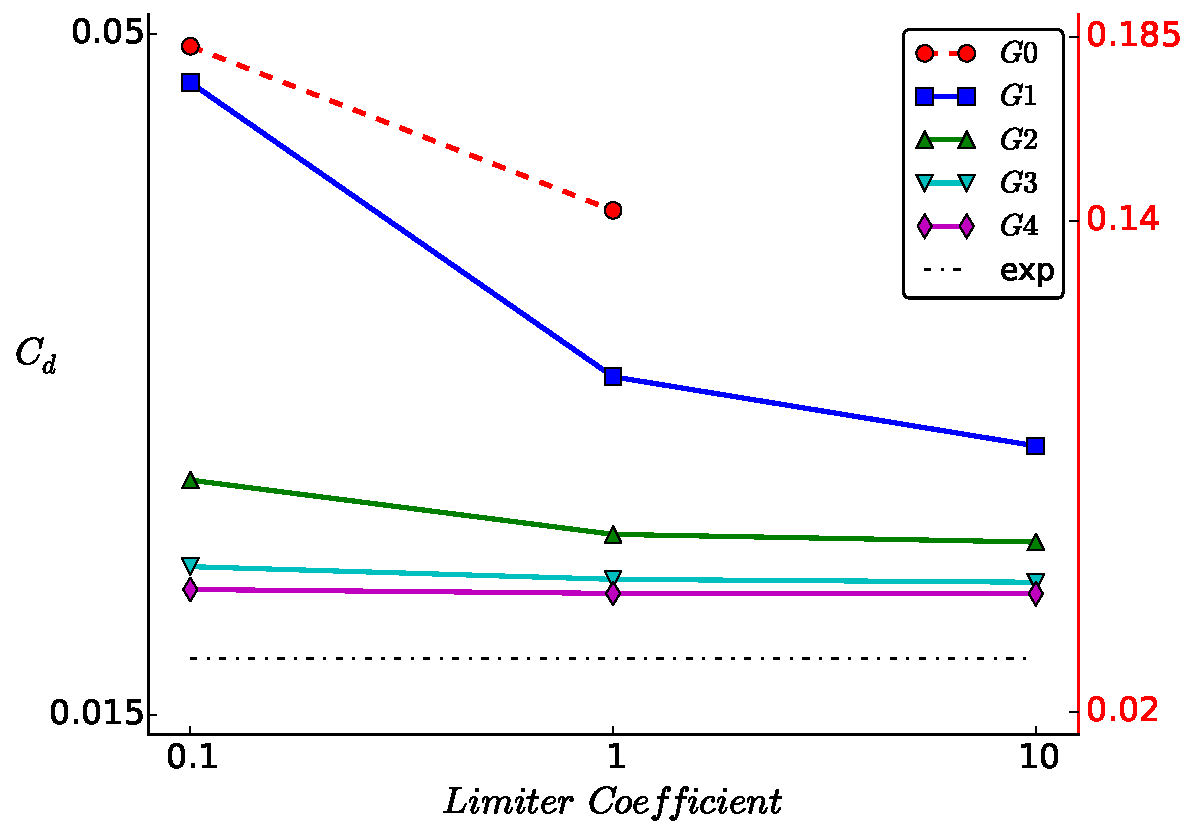
\includegraphics{limiter_vs_drag_15deg.pdf}}
        \label{fig:lim_drag_AoA15}
        \subfigure[$C_l$ Vs. limiter at $15^\circ$ Angle of Attack.]{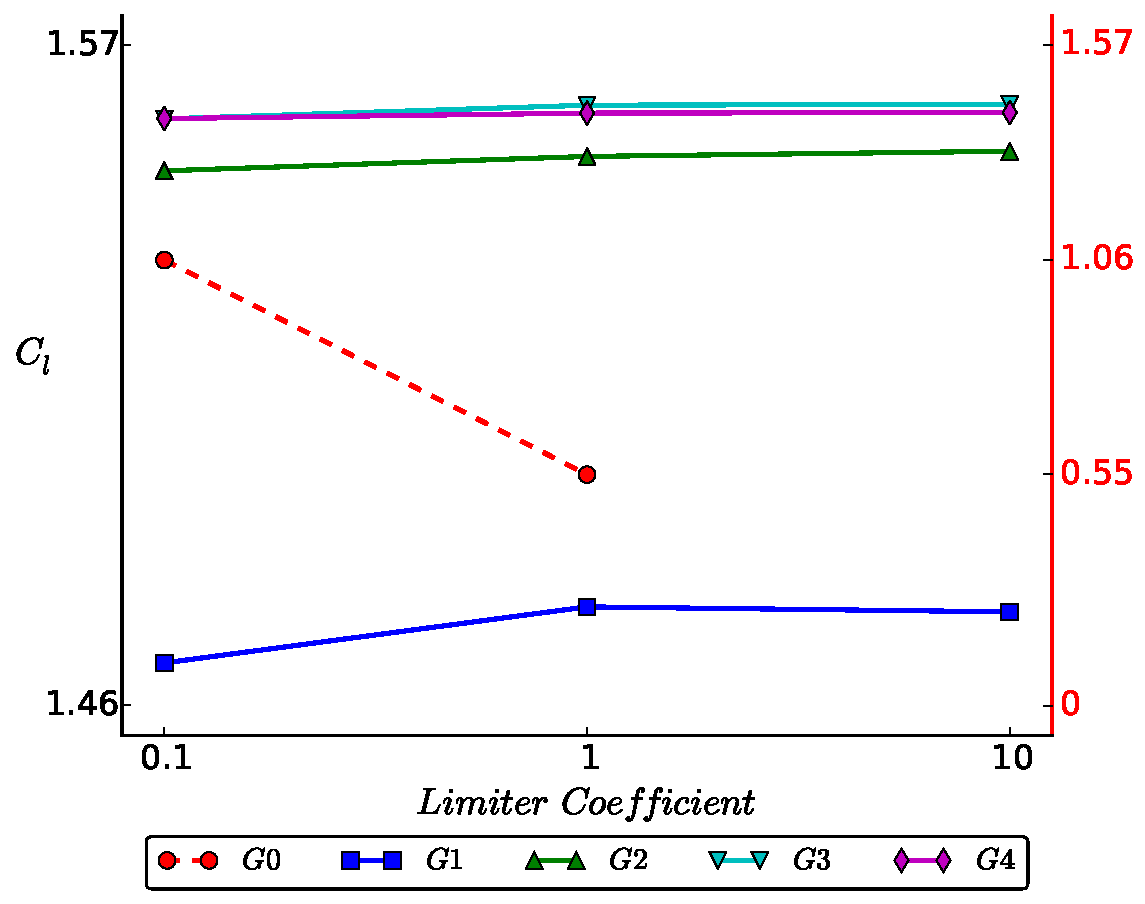
\includegraphics{limiter_vs_lift_15deg.pdf}}
        \label{fig:lim_lift_AoA15}
      \end{subfigmatrix}
  \caption{Relation between the limiter, grid resolution and integrated force coefficients for the NACA 0012. G0 results are displayed using the right hand side y-axis.}
  \label{fig:lim_grid}
\end{figure}

As can be seen from the Figure~\ref{fig:lim_grid}, the effect that the grid resolution in combination to the limiter value can be split into three categories. The first category is composed by G3 and G4, which are the finer grids and for which the limiter has little to no effect into the final converged solution. This results have been compared with available computational results and shown on Table~\ref{tab:naca_results} and are well within the range.

\begin{table}[]

  \begin{center}
  \begin{tabular}{c c c c c c c} \hline
  	\boldmath{$Contribution/Code$} & \boldmath{$C_l$}	& \boldmath{$C_l$} & \boldmath{$C_d$} & \boldmath{$C_d$} & \boldmath{$C_d$}     \\ 
  	 & \boldmath{$AoA=10$}	& \boldmath{$AoA=15$} & \boldmath{$AoA = 0$} & \boldmath{$AoA = 10$} & \boldmath{$AoA = 15$}     \\ \hline
  	
    $CFL3D$ & $1.0909$	& $1.5461$ & $0.00819$ & $0.01231$ & $0.02124$\\
    $FUN3D$ & $1.0983$	& $1.5547$ & $0.00812$ & $0.01242$ & $0.02159$\\
    $NTS$ 	& $1.0891$	& $1.5461$ & $0.00813$ & $0.01243$ & $0.02105$\\
    $JOE$ 	& $1.0918$	& $1.5490$ & $0.00812$ & $0.01245$ & $0.02148$\\
    $SUMB$  & $1.0904$	& $1.5446$ & $0.00813$ & $0.01233$ & $0.02141$\\
    $TURNS$ & $1.1000$	& $1.5642$ & $0.00813$ & $0.01233$ & $0.02140$\\
    $CGNS$  & $1.0941$	& $1.5576$ & $0.00817$ & $0.01225$ & $0.02073$\\
    $SU^2$  & $1.0988$	& $1.5577$ & $0.00801$ & $0.01277$ & $0.02264$\\
    $SU^2$ - $G4$ & $1.09644$	& $1.5578$ & $0.00810$ & $0.01236$ & $0.02146$\\
    
    
   	\hline
   	
  \end{tabular} 
  	\caption{Computational results for the NACA 0012 at RE = 6E6 and M = 0.15. $C_l$ os the lift coefficient, $C_d$ the drag coefficient and $AoA$ the angle of attack.}
  	\label{tab:naca_results}
  \end{center}
  \end{table}

The second section that comes out of the results represented on Figure~\ref{fig:lim_grid} is the middle grid range which is represented by G2. This is highly affected by the value of the limiter and as the limiter increases its effect is diminished, which allows the flow to converge towards the right solution. The upper limit of the limiter value is determined by the non-physical transient which takes place at the beginning of the simulation. The Cp plots of the NACA 0012 modeled by the G2 mesh at $15^\circ$ angle of attack are shown in Figure~\ref{fig:cp_vs_lim}. ** Describe the plots and how the higher the limiter value the closer it gets to the experimental data **

\begin{figure}[]
  \centering
    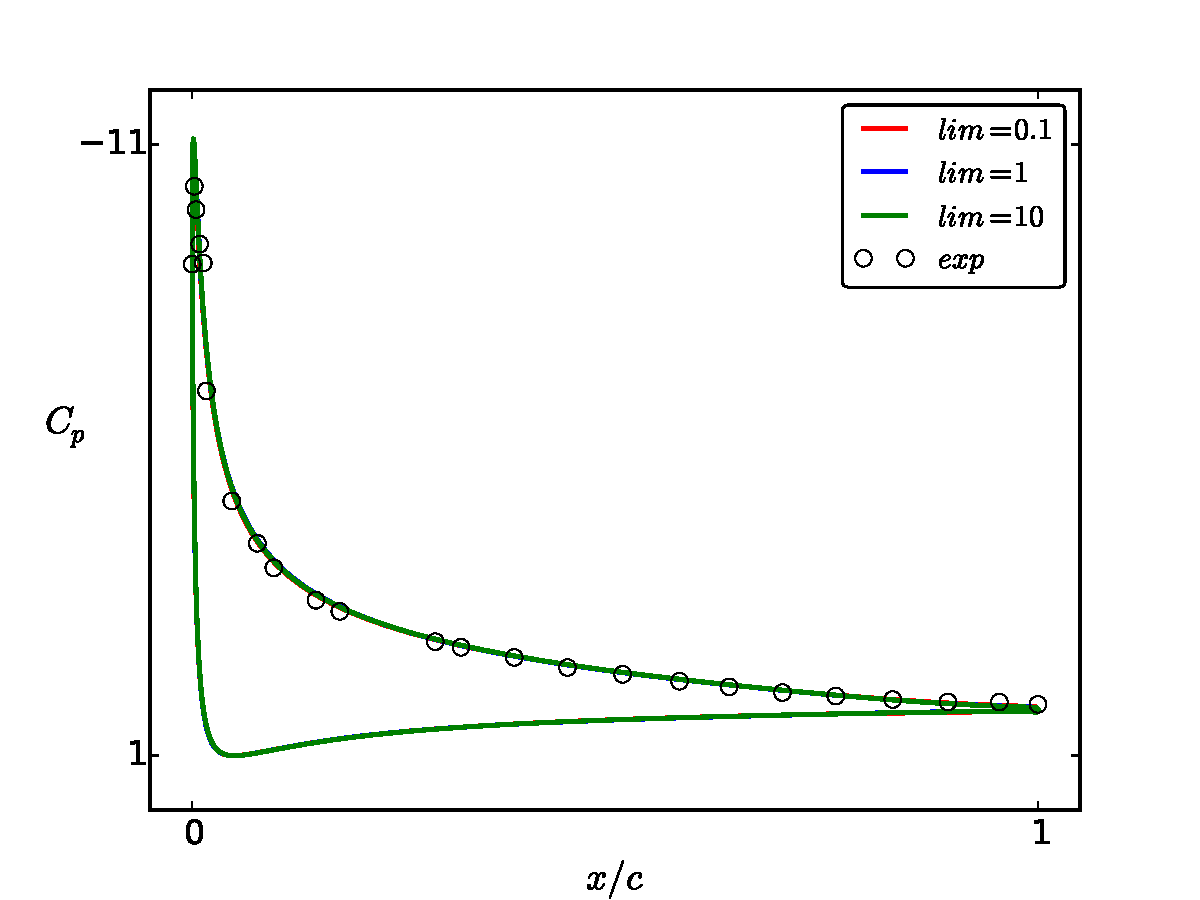
\includegraphics[width=0.5\textwidth]{Cp_vs_Lim_G2_deg15.pdf}
    \caption{Cp plots of the NACA 0012 represented by grid G2 at AoA = $15^\circ$.}
    \label{fig:cp_vs_lim}
\end{figure}

The third and final group that can be identified in Figure~\ref{fig:lim_grid} is composed by the coarse meshes G0 and G1 and care should be exercised when using them. The flow solutions obtained by using these meshes are highly dependent on the limiter value. It can be seen that as the limiter value increases, the integrated force coefficient approaches the expected solution, and to explore this trend further various limiter values were used and the results are shown in Figure~\ref{fig:limiter_exp}.

\begin{figure}[]
  \begin{subfigmatrix}{2}
    \subfigure[limiter Vs. $C_d$ for the G0 mesh.]{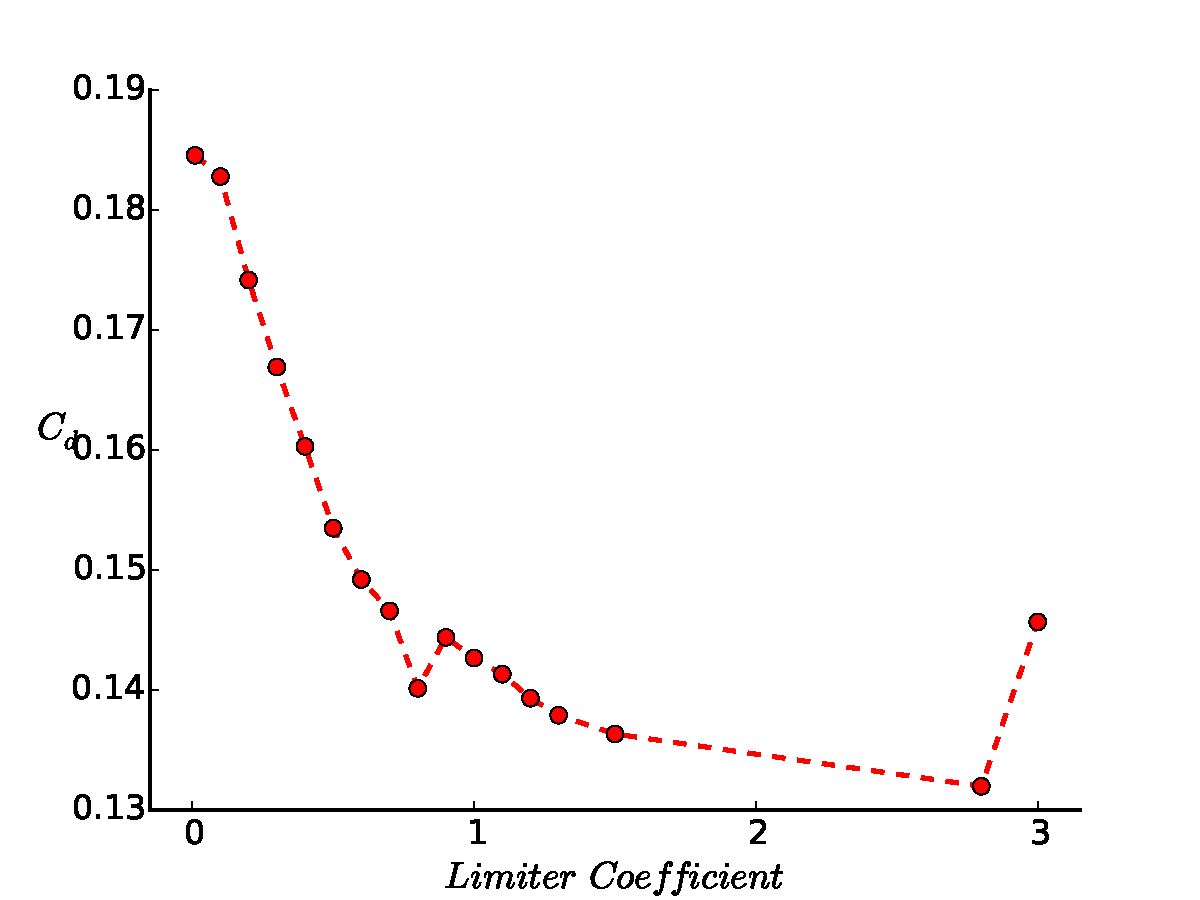
\includegraphics{G0_limiter_effect_drag15deg.pdf}}
    \label{fig:lim_cd_AoA15_G0}
    \subfigure[limiter Vs. $C_l$ for the G0 mesh.]{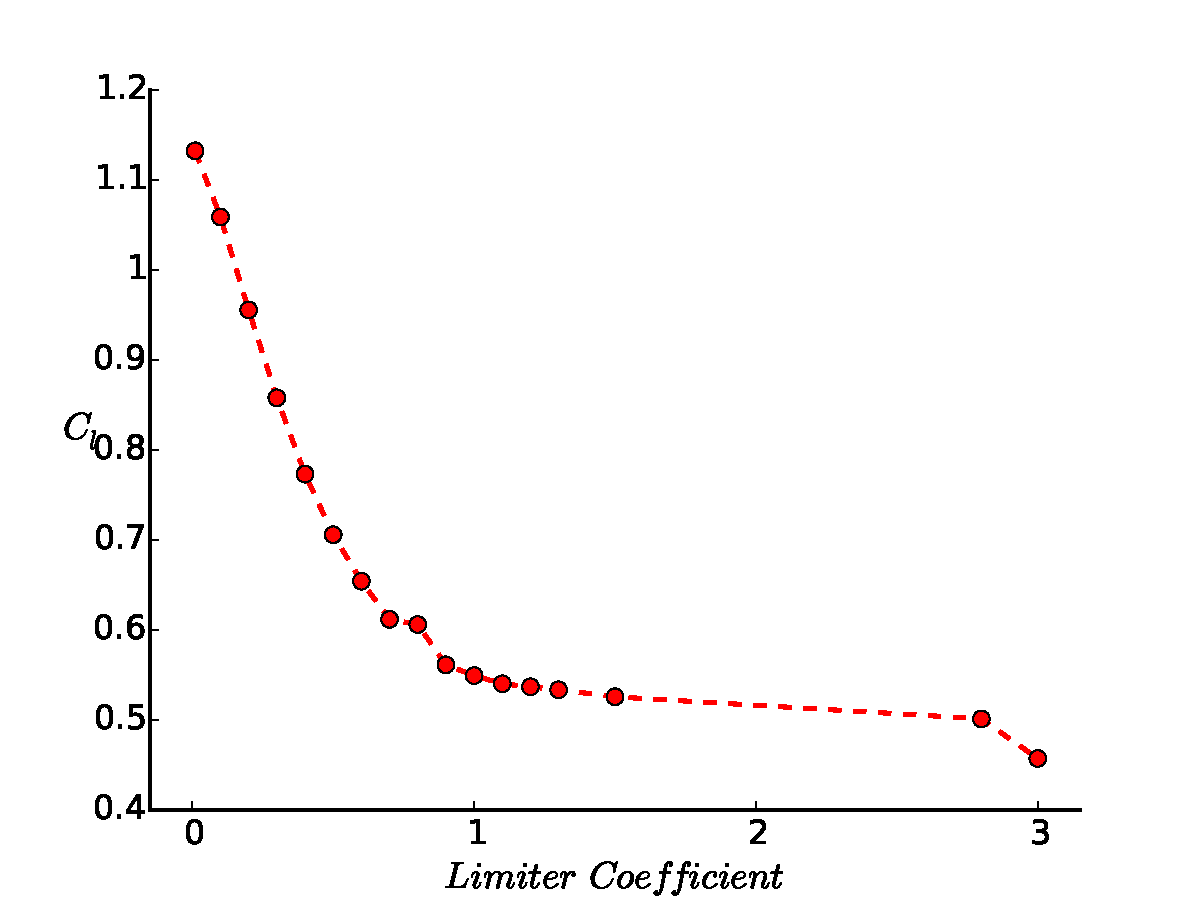
\includegraphics{G0_limiter_effect_lift15deg.pdf}}
    \label{fig:lim_cl_AoA15_G0}
  \end{subfigmatrix}
  \begin{subfigmatrix}{2}
  	\subfigure[limiter Vs. $C_d$ for the G1 mesh.]{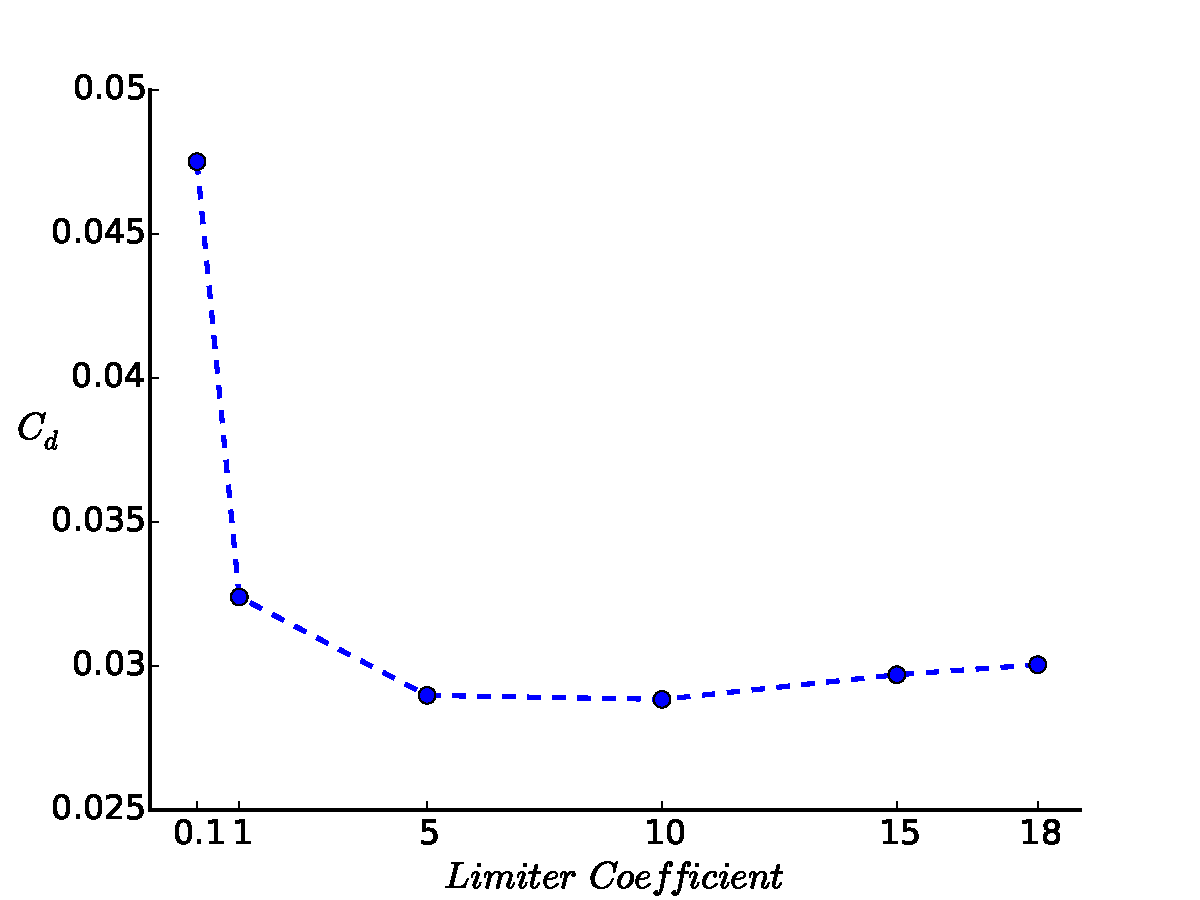
\includegraphics[width=.5\textwidth]{G1_limiter_effect_drag15deg.pdf}}
    \label{fig:lim_cd_AoA15_G1}
    \subfigure[limiter Vs. $C_l$ for the G1 mesh.]{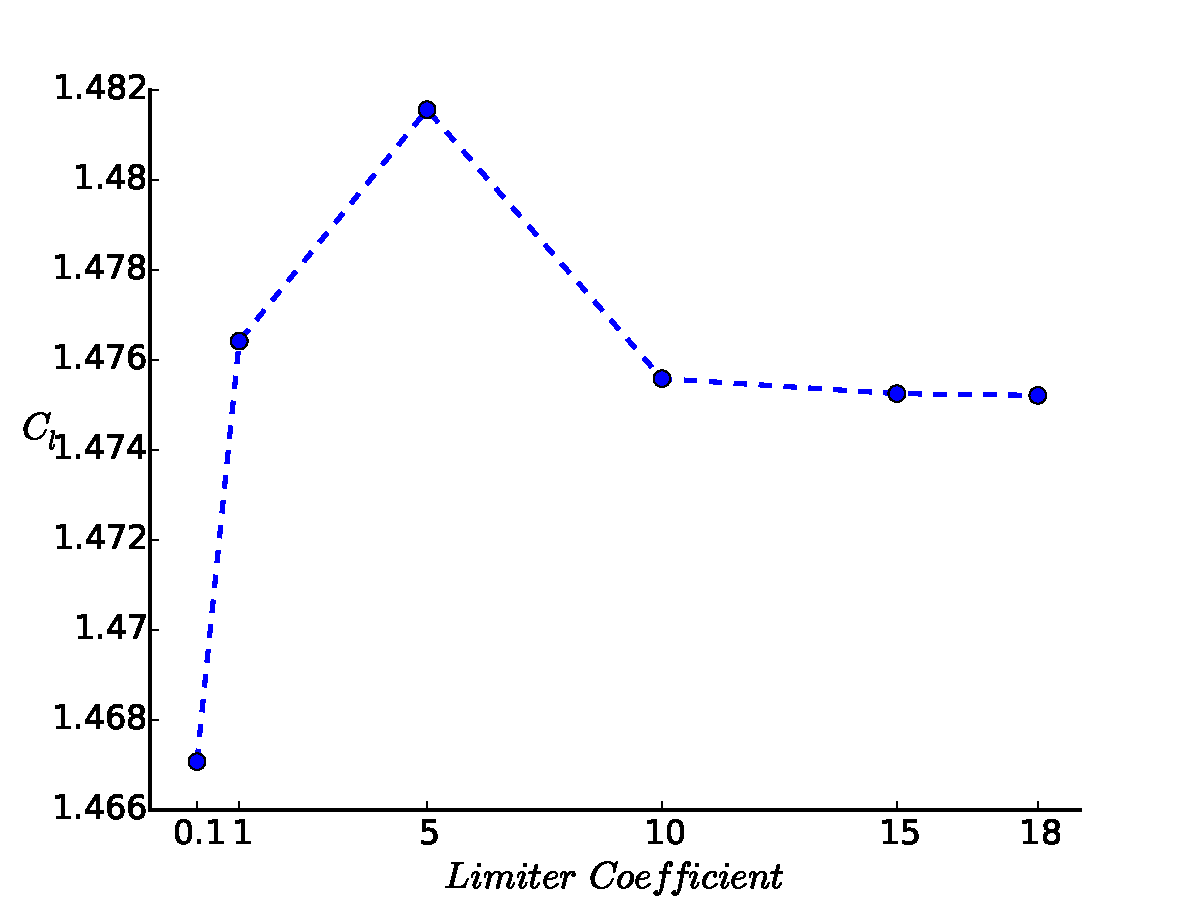
\includegraphics[width=.5\textwidth]{G1_limiter_effect_lift15deg.pdf}}
    \label{fig:lim_cl_AoA15_G1}
  \end{subfigmatrix}
  
  \caption{Limiter Vs Integrated force coefficients for the G0 and G1 meshes}
  \label{fig:limiter_exp}
\end{figure}

The G0 mesh is too coarse to be able to simulate the flow past a NACA 0012 accurately and, although the limiter has a big effect, its accuracy is limited by the mesh resolution. In the case of the G1, the integrated forces behave in a more favorable fashion and by choosing the limiter to be in the upper range, as can be seen in Figures~\ref{fig:lim_cd_AoA15_G1} and ~\ref{fig:lim_cl_AoA15_G1} one can potentially take advantage of the low computational cost while obtaining results that can be used at the first stages of shape design.

As can be clearly seen from the results show, the limiter plays a significant role in the behabior and final convergence value for coarse meshes, and to better understand the reason for this effect, the limiter value contour plot has been analyzed. 

%\begin{figure}[]
%  \begin{subfigmatrix}{2}
%    \subfigure[G0 mesh.]{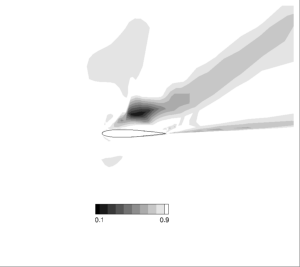
\includegraphics{lim_contour_Lim_0_1_deg15_GridG0.pdf}}
%    \label{fig:contour_G0}
%    \subfigure[G1 mesh.]{\includegraphics{lim_contour_Lim_0_1_deg15_GridG1.pdf}}
%    \label{fig:contour_G1}
%  \end{subfigmatrix}
%  \begin{subfigmatrix}{1}
%  	\subfigure[G2 mesh.]{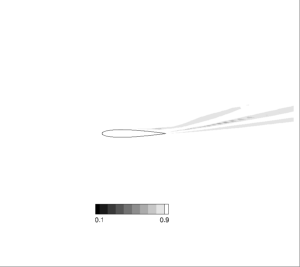
\includegraphics[width=.5\textwidth]{lim_contour_Lim_0_1_deg15_GridG2.pdf}}
%    \label{fig:contour_G2}
%  \end{subfigmatrix}

\begin{figure}[]
  \begin{subfigmatrix}{2}
    \subfigure[G0 mesh.]{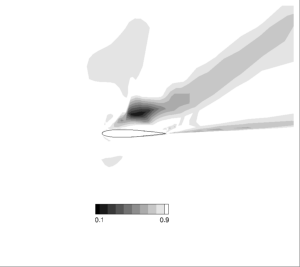
\includegraphics{lim_contour_Lim_0_1_deg15_GridG0.png}}
    \label{fig:contour_G0}
  	\subfigure[G2 mesh.]{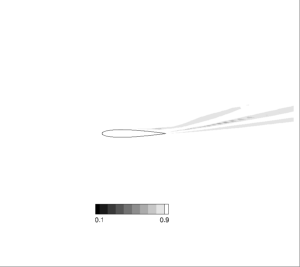
\includegraphics[width=.5\textwidth]{lim_contour_Lim_0_1_deg15_GridG2.png}}
    \label{fig:contour_G2}
  \end{subfigmatrix}
  
  \caption{Contour plot of the Venkatakrishnan limiter$\phi$ (u-velocity) for flow at AoA = $15^\circ$ with a limiter value of 0.1. }
  \label{fig:limiter_contour}
\end{figure}

** Describe the results of this three plots and come to a conclusion on the main reason for the limiters effect **

